\newcommand{\nsubparagraph}[1]{\subparagraph{\textbf{#1}}}
\newcommand{\AVG}{\mathit{AVG}}

\section{Evaluation}\label{sec:evaluation}

TODO: Some text about the section here.
% TODO: Some text about the section here.

\subsection{Experimental Setup}\label{subsec:experimentalSetup}

\begin{subequations}
    \nsubparagraph{Star Catalog:}
    The star catalog used for $K$ is the Hipparcos Input Catalogue.
    Entries that do not have a point $\left( \alpha, \delta \right)$ associated with it were not recorded, giving
    117,956 total stars.
    Out of this entire set, only 4,560 are visible from Earth with the naked eye (apparent magnitude $m$ less than 6.0).
    An additional constraint for each catalog $K^2, K^3, K^3'$ that all stars in each pair or trio be within
    $\psi < 20$ degrees of each other was placed to shorten each algorithm's query step running time.
    All sets $K^2, K^3, K^3'$ construct combinations and permutations using the 4,560 elements and this field of view
    constraint.

    Each entry in $K$ has also been updated from MJD 48319 (March 1991) to MJD 58119 (January 2018).
    The conversion to obtain these updated positions is given below:
    \begin{align}
        \alpha_t &= \alpha_\tau + \mu_\alpha (\tau - t) \\
        \delta_t &= \delta_\tau + \mu_\delta (\tau - t)
    \end{align}
    where $\mu_\alpha$ and $\mu_\delta$ represent the proper motion of some star's right ascension and declination in
    radians per year, $\alpha_\tau$ and $\delta_\tau$ represent the right ascension and declination at time
    $\tau$, $\tau$ represents the time the catalog was recorded, and $t$ represents the time we want to update
    our stars to~\cite{ProperMotion}.
    To construct the point $[ x \ y \ z ]$ for $K$,~\autoref{eq:sphereToCartesian} was used with
    each new $\left(\alpha_t, \delta_t \right)$, with $r = 1$, and then normalized.
\end{subequations}

\nsubparagraph{Benchmark Data Generation:}
Before a raw image can used in the star identification algorithms presented above, it must go through three major
processes: blob detection, centroid determination, and a 2D $\rightarrow$ 3D transformation process.
If a blob is not wholly detected, the centroid is not determined correctly, or the transformation process
is not precise enough, error will exist as input to the algorithm prior to starting.
Given that our goal is to only characterize each star identification algorithm itself, the solution implemented here
involves generating artificial images in 3D space.

Prior to generating the benchmark data, three items are specified: a field of view $\psi$, a \textit{true attitude}
$A^{\nicefrac{\iFrame}{\kFrame}}$, and a 3D vector $\vv{r_f}$ in the catalog frame $\kFrame$ that determines
the center of the image.
The next step is to find all nearby bright stars to the $\vv{r_f}$ in the catalog.
This is denoted as $J$:
\begin{equation}
    J = \set{ j \mid j \in K \land \theta\left( j, \vv{r_f} \right) < \frac{psi}{2} }
\end{equation}
To get the $I$ set, each star in $J$ is then rotated by the true attitude $A^{\nicefrac{\iFrame}{\kFrame}}$:
\begin{equation}
    I = \set{ A^{\nicefrac{\iFrame}{\kFrame}} \cdot j \mid j \in J }
\end{equation}
The set $I$, the field of view, and the rotated image center $\vv{b_f} = A^{\nicefrac{\iFrame}{\kFrame}} \cdot \vv{r_f}$
were then presented to each star identification algorithm.

The first type of noise exists as variance between the relative positions of stars represented in the catalog and those
represented in the image.
This may come from misidentifying the centroids in the image, or from out-of-date catalogs.
To introduce Gaussian noise to an image, we linearly interpolate each star toward some random 3D vector on
the unit sphere spherically (\textit{SLERP}) and distribute the magnitude of the movement normally.
To describe our noise independent of this random vector, we divide our distribution by the current angular separation
between both stars.
Given a star $b_i \in I$, Gaussian noise is applied to obtain the distributed vector $b'_i$ [CITE ME]:
\begin{equation}
    b'_i &= \frac{\sin (1 - K)\Omega}{\sin \Omega}b_i + \frac{\sin \left( K \Omega )\right}{\sin \Omega}b^\star_i
\end{equation}
where $b^\star_i$ represents some random vector whose elements are distributed uniformly, $\Omega$ describes the angle
subtended by the arc, and $K$ describes the magnitude of the interpolation:
\begin{equation}
    \begin{aligned}
        b^\star_i &= \left( \sim U(-1, 1), \sim U(-1, 1), \sim U(-1, 1) \right) \\
        \Omega &= \arccos \left ( b^{\star}_i \cdot b_i \right) \\
        K &= \frac{ \sim N\left(0, \sigma^2\right)}{\theta\left( b^{\star}_i, b_i \right)}
    \end{aligned}
\end{equation}
The additional constraint that the resulting star exist near the image center is also applied:
$\theta\left( b'_i, \vv{r_f} \right) < \nicefrac{\psi}{2}$.
If this is not met, then the process is repeated for this star.

The second type of noise exists as falsely identified sources of light, or spikes in the image.
This involves generating $b^\star_i$ in the same manner that was done for the Gaussian noise process, and normalizing
this.
If the constraint that $b^\star_i$ be near the image center is not met, this process is repeated until such a star is
found.
This is repeated for a set number of spikes.

\nsubparagraph{Hardware:}
All trials were performed on an Intel i7-7700 CPU, 3.60GHz with 8 GB RAM\@.
Each algorithm was implemented in C++14, and compiled without optimization (at \texttt{-O0}).
The exact implementation is available at the following link:
\url{https://github.com/glennga/hoku}.

\subsection{1st Filter: Catalog}\label{subsec:1stFilter:Catalog}
\nsubparagraph{Determining Query $\sigma$:} TODO: Some text here % TODO: Finish this part

The results of each grid search are displayed below, and were used for the following experiments.
\begin{alignat*}{3} % TODO: Format this with \num?
    \text{Angle}&: \sigma_\theta &&= 10^{-4} &&{}\\
    \text{Pyramid}&: \sigma_\theta &&= 10^{-4} &&{} \\
    \text{Dot Angle}&: \sigma_{\theta_{c1}} &&= 10^{-2}, \sigma_{\theta_{c2}} &&= 10^{-2}, \sigma_\phi = 10^{-2} \\
    \text{Spherical Triangle}&: \sigma_a &&= 10^{-9}, \sigma_\imath &&= 10^{-9} \\
    \text{Planar Triangle}&: \sigma_a &&= 10^{-9}, \sigma_\imath &&= 10^{-9} \\
    \text{Composite Pyramid}&: \sigma_a &&= 10^{-9}, \sigma_\imath &&= 10^{-9}
\end{alignat*}

\begin{table}
    \centering {
    %\begin{tabular}{m{0.22\columnwidth}|m{0.2\columnwidth}|m{0.2\columnwidth}|m{0.2\columnwidth}} \toprule
%    \textit{Method} & $y'$ & $S$ & $t_{\AVG} \ (\si{ms})$  \\ \hline
%    Angle & \num{2000} & \num{32} & \num{138.00} \\ \hline
%    Interior Angle & \num{2000} & \num{1440} & \num{171.80} \\ \hline
%    Planar \newline Triangle & \num{2000} & \num{1994} & \num{139.05} \\ \hline
%    Composite \newline Pyramid & \num{2000} & \num{1991} & \num{139.46} \\ \hline
%    Spherical \newline Triangle & \num{2000} & \num{1984} & \num{139.60} \\ \hline
%    Pyramid & \num{1980} & \num{1501} & \num{149.69} \\ \bottomrule
%\end{tabular}

\begin{tabular}{m{0.22\columnwidth}|m{0.2\columnwidth}|m{0.2\columnwidth}|m{0.2\columnwidth}}
    \toprule
    \textit{Method} & $f_{r_b \in R}$ & $S$ & $t_{\AVG} \ (\si{ms})$  \\ \hline
    ANG & \num{1.0} & \num{32} & \num{138.00} \\ \hline
    INT & \num{1.0} & \num{1440} & \num{171.80} \\ \hline
    PLN / COM & \num{1.0} & \num{1994} & \num{139.05} \\ \hline
%    Composite \newline Pyramid & \num{1.0} & \num{1991} & \num{139.46} \\ \hline
    SPH & \num{1.0} & \num{1984} & \num{139.60} \\ \hline
    PYR & \num{0.99} & \num{1501} & \num{149.69} \\ \bottomrule
\end{tabular}
    \caption{
    Depicts all data associated with testing the query step: the probability that the correct catalog set ($r_b$,
    such that the correct bijection can be formed with $b$) exists in $R$ after querying, the number of trials where the
    resulting $R$ meets the $\abs{R} = 1$ criterion ($S$),
    and the average query running time ($t_{\AVG}$) given images with no noise.
    There exist 2000 runs for each identification method.
    } \label{tab:queryExperimentResults}
    }
\end{table}

\subsubsection{Which method has the fastest catalog query step?}
In~\autoref{sec:starIdentificationMethods}, we describe each method's running time in terms of the number of catalog
accesses $n$ and the size of the $K^d$ catalog.
The $K^2$ catalog, used by the Angle and Pyramid methods, is of size $m_2 = 353,700$ elements with the apparent
magnitude and field-of-view constraints.
The $K^3$ catalog, used by the Spherical Triangle, Planar Triangle, and Composite Pyramid methods is of size
$m_3 = 12,520,359$ elements.
The $K^3'$ catalog, used by the Dot Angle method is of size $m_{3'} = 37,561,083$ elements.
Given the size of each catalog, we hypothesize that the Angle method has the fastest query step
(Pyramid method accesses $K^2$ three times in query step) and the Dot Angle has the slowest query step.

In~\autoref{tab:queryExperimentResults}, the average running time to obtain an $R$ set is displayed for each
identification method given an image for 2000 runs.
The slowest method on average is the Dot Angle method, with its $t_{\AVG} = 30.64 \si{ms}$ longer than the average
$t_{\AVG}$ for all other methods ($30.64 \pm 4.30 \si{ms}$).
Given that this method has the largest catalog, more time should be spent searching for the appropriate elements.

%# http://www.socscistatistics.com/pvalues/normaldistribution.aspx
%import numpy as np
%m_1, m_2, s_1, s_2, n_1, n_2 = 137.9965, 139.051, 4.201486373891982, 3.3748183654828003, 2000, 2000
%z_plane = (m_2 - m_1) / np.sqrt( ((s_1 * s_1) / n_1) + ((s_2 * s_2) / n_2) )
We note that the two fastest methods appear to be Angle method and the Planar Triangle method, but their $t_\AVG$ only
vary by 1.05ms.
Given the null hypothesis that the difference between the Planar Triangle method's query step running time and the
Angle method's query step running time is not significant, $z = 8.75, p < 0.0001$ is found with a two-tailed two
sample $Z$ test.
The running times are very likely not equal.
With the data collected here, the Angle method has the fastest query step.

\subsubsection{Which method meets the $\abs{R} = 1$ criterion the most often?}
The $\abs{R} = 1$ criterion is required for all identification methods, and meeting this criteria as often as possible
prevents additional catalog accesses from occurring.
In~\autoref{tab:queryExperimentResults}, the lowest number of instances where the criterion is met $S$ lies with the
Angle method.
Out of 2000 query steps, the Angle method will have had to perform an additional query step at least 1968 more times.
The Pyramid method only has 499 of these additional query instances, which is a factor of 3.94 less.
The most likely reason for this lies with the selection of the $\sigma_\theta$ parameter, and the fact that only one
feature is used to query $K^2$.
If $\sigma_\theta$ was chosen to be smaller, there would have been more instances where the criterion was met- but
this comes at the cost of being less flexible with Gaussian noise.
The methods using $K^3$ and $K^3'$ have the advantage of being able to create utilize more features of the $b$ set and
distinguish it better, compared to only using $\theta(b, r)$ as the sole feature.

%import numpy as np
%p_1, p_2, n_1, n_2 = (1501 / 2000), ((1994 + 1991 + 1984) / 6000), 2000, 6000
%p = (1501 + 1994 + 1991 + 1984) / (2000 + 6000)
%z = (p_2 - p_1) / np.sqrt( p * (1 - p) * ((1/n_1) + (1/n_2)) )
It appears that the all methods using triangular features (Planar Triangle, Composite Pyramid, Spherical Triangle)
meet the criterion the most often (average of $1989.7 \pm 4.2$ runs).
Again, a larger $\sigma_a$ or $\sigma_\imath$ query parameter may lead to a larger $\abs{R}$.
The next method with the most $\abs{R} = 1$ runs that does not use triangular features is the Pyramid method.
Given the null hypothesis that the difference between the number of $\abs{R} = 1$ Pyramid method runs and the
number of $\abs{R} = 1$ runs for methods with triangular features is not significant, $z = 38.0, p < 0.0001$ is
obtained with a two proportion $Z$ test.
With the data collected here, we find that methods with triangular features are very likely to have more instances
where the $\abs{R} = 1$ criterion is met.

\subsubsection{How effective is the Pyramid method query?}
In the Angle, Spherical Triangle, Planar Triangle, and Composite Pyramid methods, catalog queries can be
generalized to the following SQL query:
\begin{align*}
    \texttt{SELECT } &r \\
    \texttt{FROM } &K^d \\
    \texttt{WHERE } &g_1(r) < g_1(b) + 3\sigma_{g1} \texttt{ AND } g_1(r) > g_1(b) - 3\sigma_{g1} \texttt{ AND } \\
    &g_2(r) < g_2(b) + 3\sigma_{g2} \texttt{ AND } g_2(r) > g_2(b) - 3\sigma_{g2} \\
    &\vdots \\
    &g_d(r) < g_d(b) + 3\sigma_{gd} \texttt{ AND } g_d(r) > g_d(b) - 3\sigma_{gd}
\end{align*}
\begin{align*}
    d =& \text{ number of stars used in the query.} \\
    g =& \text{ function used to obtain a feature. } \\
    \sigma =& \text{ deviation of noise. }
\end{align*}
The Dot Angle method requires the $\theta(r_{c1}, r_{c}) < \theta(r_{c2}, r_c)$ constraint before performing the query
above, but the Pyramid method has the most involved query that involves processing outside of SQL\@.
Three of the queries above must be performed to obtain several different $R$ sets, and the common stars must be
found among each $R$ set to create a singular candidate set for trios.

%# http://www.socscistatistics.com/pvalues/normaldistribution.aspx
%import numpy as np
%m_1, m_2, s_1, s_2, n_1, n_2 = 0.99, 1.0, 0.09949874371066202, 0, 2000, 2000
%z = (m_2 - m_1) / np.sqrt( ((s_1 * s_1) / n_1) + ((s_2 * s_2) / n_2) )
There exist several areas where the Pyramid could drop in accuracy here.
In~\autoref{tab:queryExperimentResults}, the frequency of the correct $r$ for some $b$ existing in $R$ is displayed
for each identification method.
The Pyramid method is shown to have a 0.01\% difference from the 100\% accuracy of each other method.
Given the null hypothesis that this difference is not significant, $z= 4.49, p < 0.0001$ is obtained with a one tailed
two sample $Z$ test.
With the data collected here, we find that the Pyramid method's query step is less accurate than other identification
methods.
Although small, this error will propagate to the next steps and will result in more catalog accesses.

\subsection{2nd Filter: Catalog Candidates}\label{subsec:2ndFilter:CatalogCandidates}
\begin{figure}
    \centering{
    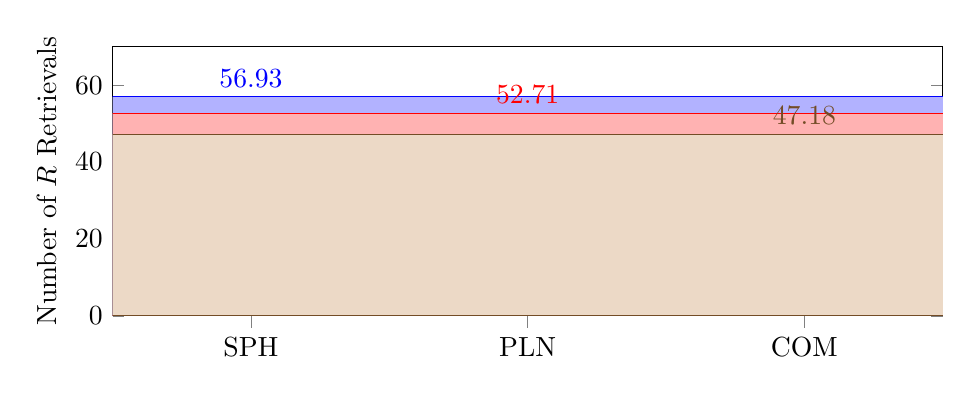
\begin{tikzpicture}
    \begin{axis}[
    ybar,
    width=\linewidth, height=5cm,
    ylabel={Number of $R$ Retrievals}, ylabel near ticks, ymin=0, ymax=70,
    xticklabels={SPH, PLN, COM},
    xtick={1, 2, 3}, xmin=0.5, xmax=3.5, xtick pos=left,
    nodes near coords, nodes near coords align={vertical},
    every axis plot/.append style={
    ybar,
    bar width=40,
    bar shift=0pt,
    fill
    }
    ]
        \addplot coordinates {(1, 56.93)}; % SPH
        \addplot coordinates {(2, 52.71)}; % PLN
        \addplot coordinates {(3, 47.18)};
    \end{axis}
\end{tikzpicture}

%SELECT AVG(QueryCount), IdentificationMethod
%FROM REDUCTION
%WHERE rowid IN (
%    SELECT rowid
%    FROM REDUCTION
%    WHERE (IdentificationMethod LIKE 'Plane' OR IdentificationMethod LIKE 'Sphere')
%    AND ShiftDeviation < 1.0e-3 AND ShiftDeviation > 1.0e-5 AND FalseStars = 0
%    AND QueryCount > 1
%)
%GROUP BY IdentificationMethod

%SELECT AVG(QueryCount)
%FROM REDUCTION
%WHERE rowid IN (
%    SELECT rowid
%    FROM REDUCTION
%    WHERE IdentificationMethod LIKE 'Composite'
%    AND ShiftDeviation < 1.0e-3 AND ShiftDeviation > 1.0e-5 AND FalseStars = 0
%    AND QueryCount > 1
%)
    \caption{
    Depicts the average number of catalog accesses required to obtain a $r$ set for methods with triangular
    features given $\sigma = \ang{0.0001}$ of Gaussian noise.
    To characterize the pivoting method itself, we only display instances where $\abs{R} \neq 1$ with the first $b$
    selection.
    The Spherical Triangle method (SPH) has 1952 / 2000 runs matching the criteria before, the Planar Triangle
    method (PLN) has 1946 runs, and the Composite Pyramid (COM) method has 1957 runs.
    }\label{fig:rPivot}
    }
\end{figure}

\subsubsection{How expensive is the pivoting process?}
%import numpy as np
%m_1, m_2, s_1, s_2, n_1, n_2 = 52.71, 47.18, 56.794658219949106, 47.01765577951369, 1946, 1957
%z = (m_2 - m_1) / np.sqrt( ((s_1 * s_1) / n_1) + ((s_2 * s_2) / n_2) )
As seen previously, identification methods with triangular features have the most number of instances where
$\abs{R} = 1$ given an image with no noise.
In~\autoref{fig:rPivot}, the average number of catalog accesses are displayed for these same methods where the first
$b$ selection does not meet the $R$ criterion given an image with Gaussian noise.
We note that the average number of catalog accesses is higher in methods that use the pivoting processes,
as opposed to those that do not.
Given the null hypothesis that the difference between the Planar Triangle method's number of catalog accesses and
the Composite Pyramid method's number of catalog accesses is not significant, $z = 3.3, p < 0.0001$ is
obtained with a two-tailed two sample $Z$ test.
With the data collected here, we find that the pivoting process results in more catalog accesses on average.
This results in a $6.70\si{ms}$ difference on average between the two.

The pivoting process was only tested with methods using triangular features, whose candidate sets met the $R$ criterion
the most frequently.
An area of interest would be to see the effects of applying this process to methods with angular features (i.e.\ Angle,
Dot Angle, Pyramid).
These methods met the criterion less frequently, and would likely benefit from attempting to reduce the $R$ set before
deciding to choose another $b$ set.

\section{End to End}\label{sec:endToEndEvaluation}

\begin{figure*}
    \centering{
    \begin{subfigure}[b]{0.48\linewidth}
        \begin{tikzpicture}
    \begin{axis}[
    ybar,
    width=\linewidth, height=5cm,
    ylabel={$t \ (\si{ms})$}, ylabel near ticks, ymin=10, ymax=100000,
    xtick={1, 2, 3}, xticklabels={$\ang{0}$, $\ang{0.0001}$, $\ang{0.01}$},
    xlabel={$\sigma$ (degrees)}, xmin=0.5, xmax=3.5, xtick pos=left, point meta=rawy,
    nodes near coords, every node near coord/.append style={rotate=90, anchor=west,
    /pgf/number format/.cd,fixed,precision=6},
    legend style={at={(0.5,-0.35)}, anchor=north,legend columns=-1},
    bar width=7, ymode=log, log origin=infty, max space between ticks=20
    ]
        \addplot coordinates {(1, 1197.43) (2, 1349.07) (3, 6509.00)};
        \addplot coordinates {(1, 160.68) (2, 161.80) (3, 872.22)};
        \addplot coordinates {(1, 323.94) (2, 339.23) (3, 392.29)};
        \addplot coordinates {(1, 324.35) (2, 328.85) (3, 352.24)};
        \addplot coordinates {(1, 170.79) (2, 171.53) (3, 364.04)};
        \addplot coordinates {(1, 405.53) (2, 1545.45) (3, 362.30)};
        \legend{ANG, INT, SPH, PLN, PYR, COM}
    \end{axis}
\end{tikzpicture}
    \end{subfigure}
    \begin{subfigure}[b]{0.48\linewidth}
        \begin{tikzpicture}
    \begin{axis}[
    ybar,
    width=\linewidth, height=5cm,
    ylabel={$a(h, b, r)$}, ylabel near ticks, ymin=0, ymax=1.3,
    xtick={1, 2, 3}, xticklabels={$\ang{0}$, $\ang{0.0001}$, $\ang{0.01}$},
    xlabel={$\rho$ (degrees)}, xmin=0.5, xmax=3.5, xtick pos=left,
    nodes near coords, every node near coord/.append style={rotate=90, anchor=west},
    legend style={at={(0.5,-0.35)}, anchor=north,legend columns=-1},
    bar width=7
    ]
        \addplot coordinates {(1, 0.977) (2, 0.973) (3, 0.004)};
        \addplot coordinates {(1, 1.0) (2, 1.0) (3, 0.706)};
        \addplot coordinates {(1, 1.0) (2, 0.814) (3, 0.025)};
        \addplot coordinates {(1, 1.0) (2, 0.862) (3, 0.025)};
        \addplot coordinates {(1, 0.999) (2, 0.999) (3, 0)};
        \addplot coordinates {(1, 1.0) (2, 0.003) (3, 0)};
        \legend{ANG, INT, SPH, PLN, PYR, COM}
    \end{axis}
\end{tikzpicture}
    \end{subfigure}
    \caption{
    Both plots represent some statistic about the resulting bijection $f$ produced by each identification method
    given some image with varying Gaussian noise.
    The left plot depicts the average time to obtain $f$, and the right plot depicts the average accuracy of $f$.
    There exist 2000 runs for each identification method, with a 500 $b$ selection bound.
    }\label{fig:gaussianNoise}
    }
\end{figure*}

\begin{figure*}
    \centering{
    \begin{subfigure}[b]{0.48\linewidth}
        \begin{tikzpicture}
    \begin{axis}[
    ybar,
    width=\linewidth, height=5cm,
    ylabel={$t \ (\si{ms})$}, ylabel near ticks, ymin=10, ymax=100000,
    xtick={1, 2, 3}, xticklabels={0, 6, 12},
    xlabel={$\omega$}, xmin=0.5, xmax=3.5, xtick pos=left, point meta=rawy,
    nodes near coords, every node near coord/.append style={rotate=90, anchor=west,
    /pgf/number format/.cd,fixed,precision=2},
    legend style={at={(0.5,-0.35)}, anchor=north,legend columns=-1},
    bar width=7, ymode=log, log origin=infty, max space between ticks=20
    ]
        \addplot coordinates {(1, 1197.43) (2, 1737.94) (3, 2431.58)};
        \addplot coordinates {(1, 160.68) (2, 209.36) (3, 280.54)};
        \addplot coordinates {(1, 323.94) (2, 355.54) (3, 386.20)};
        \addplot coordinates {(1, 324.35) (2, 350.60) (3, 390.41)};
        \addplot coordinates {(1, 170.79) (2, 183.71) (3, 195.53)};
        \addplot coordinates {(1, 405.53) (2, 685.07) (3, 972.04)};
        \legend{ANG, DOT, SPH, PLN, PYR, COM}
    \end{axis}
\end{tikzpicture}
    \end{subfigure}
    \begin{subfigure}[b]{0.48\linewidth}
        \begin{tikzpicture}
    \begin{axis}[
    ybar,
    width=\linewidth, height=5cm,
    ylabel={$a(f, b, r)$}, ylabel near ticks, ymin=0, ymax=1.4,
    xtick={1, 2, 3}, xticklabels={0, 6, 12},
    xlabel={$\omega$}, xmin=0.5, xmax=3.5, xtick pos=left,
    nodes near coords, every node near coord/.append style={rotate=90, anchor=west,
    /pgf/number format/.cd,fixed,precision=4},
    legend style={at={(0.5,-0.35)}, anchor=north,legend columns=-1},
    bar width=7
    ]
        \addplot coordinates {(1, 0.977) (2, 0.979) (3, 0.960)};
        \addplot coordinates {(1, 1.0) (2, 0.982) (3, 0.965)};
        \addplot coordinates {(1, 1.0) (2, 0.840) (3, 0.696)};
        \addplot coordinates {(1, 1.0) (2, 0.845) (3, 0.703)};
        \addplot coordinates {(1, 0.999) (2, 0.999) (3, 0.995)};
        \addplot coordinates {(1, 1.0) (2, 0.994) (3, 0.973)};
        \legend{ANG, DOT, SPH, PLN, PYR, COM}
    \end{axis}
\end{tikzpicture}
    \end{subfigure}
    \caption{
    Both plots represent some statistic about the resulting bijection $f$ produced by each identification method
    given some image with varying amounts of spikes (false stars).
    The left plot depicts the average time to obtain $f$, and the right plot depicts the average accuracy of $f$.
    There exist 2000 runs for each identification method, with a 500 $b$ selection bound.
    }\label{fig:falseNoise}
    }
\end{figure*}

\subsubsection{Which method is the most accurate under Gaussian noise?}

\subsubsection{Which method is the fastest under Gaussian noise?}

\subsubsection{Which method is the most accurate under false star noise?}

\subsubsection{Which method is the fastest under false star noise?}